\documentclass[aspectratio=169]{beamer}
\usetheme[]{msubeamer}
\usepackage[T1]{fontenc}
% BACKGROUND CHOICES: windows(default),chevron,diamonds,antique,circles,ornate,eyes,hexagons

\usepackage{multicol, bibentry}
\usepackage[backend=bibtex,sorting=none]{biblatex}
\addbibresource{D2GM.bib} 
\newcounter{mycounter}
\usepackage[latin1]{inputenc}
\usepackage{movie15}
%\usepackage{authblk}
\usepackage{graphicx}
\usepackage{lipsum}
\usepackage{multirow}
\usepackage{amsfonts}
\usepackage{subfigure}
\usepackage{graphicx}
\usepackage{epstopdf}
\usepackage{color}
\usepackage{float}
\usepackage{tikz} 
\usepackage{amsmath}
\usepackage{multirow}
\usetikzlibrary{positioning,datavisualization,datavisualization.formats.functions}
\usepackage{amssymb,mathrsfs,MnSymbol}%,skak}
\usepackage{amsthm}
%%
%\usepackage[ngerman]{babel}
\usepackage[T1]{fontenc}
\usepackage{graphicx,graphics}
\usepackage{pgf}
\usepackage{colortbl}
\usepackage[english]{babel}
\usepackage{rotating}
\usepackage{subfigure}
\usepackage{tikz}
%%%%%%%%%%%%%%%%%%%%%%%%%%%%%%%%%%%%%%MACROS

\def\bb {\mathbf{b}}
\def\bC {\mathbf{C}}
\def\bD {\mathbf{D}}
\def\bE {\mathbf{E}}
\def\bF {\mathbf{F}}
\def\bG {\mathbf{G}}
\def\bh {\mathbf{h}}
\def\bH {\mathbf{H}}
\def\bI {\mathbf{I}}
\def\bK {\mathbf{K}}
\def\bm {\mathbf{m}}
\def\bn {\mathbf{n}}
\def\bN {\mathbf{N}}
\def\bp {\mathbf{p}}
\def\bP {\mathbf{P}}
\def\bq {\mathbf{q}}
\def\bQ {\mathbf{Q}}
\def\bR {\mathbf{R}}
\def\bS {\mathbf{S}}
\def\bT {\mathbf{T}}
\def\bV {\mathbf{V}}
\def\bv {\mathbf{v}}
\def\bw {\mathbf{w}}
\def\bW {\mathbf{W}}
\def\bx {\mathbf{x}}
\def\bxi {\mathbf{xi}}
\def\bz {\mathbf{z}}
\def\bZ {\mathbf{Z}}
\def\ff {\mathbf{f}}
\def\btheta {\mathbf{\theta}}

\def\bbE {\mathbb{E}}
\def\bbR {\mathbb{R}}
\def\bbZ {\mathbb{Z}}


\def\fA {\mathfrak{A}}
\def\fH {\mathfrak{H}}
\def\fS {\mathfrak{S}}
\def\fZ {\mathfrak{Z}}

\def\cA {\mathcal{A}}
\def\cB {\mathcal{B}}
\def\cC {\mathcal{C}}
\def\cD {\mathcal{D}}
\def\cE {\mathcal{E}}
\def\cF {\mathcal{F}}
\def\cG {\mathcal{G}}
\def\cH {\mathcal{H}}
\def\cI {\mathcal{I}}
\def\cJ {\mathcal{J}}
\def\cK {\mathcal{K}}
\def\cL {\mathcal{L}}
\def\cM {\mathcal{M}}
\def\cN {\mathcal{N}}
\def\cP {\mathcal{P}}
\def\cQ {\mathcal{Q}}
\def\cR {\mathcal{R}}
\def\cS {\mathcal{S}}
\def\cT {\mathcal{T}}
\def\cU {\mathcal{U}}
\def\cV {\mathcal{V}}
\def\cW {\mathcal{W}}
\def\cX {\mathcal{X}}
\def\cZ {\mathcal{Z}}

\def\scrA{\mathscr{A}}
\def\scrB{\mathscr{B}}
\def\scrC{\mathscr{C}}
\def\scrE{\mathscr{E}}
\def\scrH{\mathscr{H}}
\def\scrL{\mathscr{L}}
\def\scrM{\mathscr{M}}

\def\scrR{\mathscr{R}}
\def\scrV{\mathscr{V}}

\def\a {{\alpha}}
\def\b {{\beta}}
\def\g {{\gamma}}
\def\Ga {{\Gamma}}
\def\de {{\delta}}
\def\eps {{\epsilon}}
\def\th {{\theta}}
\def\io {{\iota}}
\def\ka {{\kappa}}
\def\l {{\lambda}}
\def\L {{\Lambda}}
\def\si {{\sigma}}
\def\Si {{\Sigma}}
\def\Ups {{\Upsilon}}
\def\tUps {{\tilde\Upsilon}}
\def\om {{\omega}}
\def\bom{{\mathbf{\omega}}}
\def\Om {{\Omega}}

\def\d {{\partial}}
\def\grad {{\nabla}}
\def\Dlt {{\Delta}}

\def\rstr {{\big |}}
\def\indc {{\bf 1}}

\def\wtilde {\widetilde }
\def\what {\widehat }

\def\la {\langle}
\def\ra {\rangle}
\def \La {\bigg\langle}
\def \Ra {\bigg\rangle}
\def \lA {\big\langle \! \! \big\langle}
\def \rA {\big\rangle \! \! \big\rangle}
\def \LA {\bigg\langle \! \! \! \! \! \; \bigg\langle}
\def \RA {\bigg\rangle \! \! \! \! \! \; \bigg\rangle}

\def\pp {{\parallel}}

\def\vide {{\varnothing}}

\def\wL {{w-L}}
\def\wto {{\rightharpoonup}}

\def\Sh {{\hbox{S\!h}}}
\def\Kn{{\hbox{K\!n}}}
\def\Ma{{\hbox{M\!a}}}
\def\Rey{{\hbox{R\!e}}}

\def\bFc {{\bF^{\hbox{conv}}_\eps}}
\def\bFcn{{\bF^{\hbox{conv}}_{\eps_n}}}
\def\bFd {{\bF^{\hbox{diff}}_\eps}}
\def\bFdn{{\bF^{\hbox{diff}}_{\eps_n}}}

\def\DDS {\mathcal{D}_{Slater}}
\def\De {{_\eta D}}

\def\bu {{\bullet}}
\def\dd {\,\mathrm{d}}

\newcommand{\vvec}{\overrightarrow}
\newcommand{\Div}{\operatorname{div}}
\newcommand{\Rot}{\operatorname{curl}}
\newcommand{\Diam}{\operatorname{diam}}
\newcommand{\Dom}{\operatorname{Dom}}
\newcommand{\Sign}{\operatorname{sign}}
\newcommand{\Span}{\operatorname{span}}
\newcommand{\Supp}{\operatorname{supp}}
\newcommand{\Det}{\operatorname{det}}
\newcommand{\Tr}{\operatorname{trace}}
\newcommand{\Codim}{\operatorname{codim}}
\newcommand{\Dist}{\operatorname{dist}}
\newcommand{\DDist}{\operatorname{Dist}}
\newcommand{\Ker}{\operatorname{Ker}}
\newcommand{\IM}{\operatorname{Im}}
\newcommand{\Id}{\operatorname{Id}}
\newcommand{\Lip}{\operatorname{Lip}}
\newcommand{\Osc}{\operatorname{osc}}
\newcommand{\Esssup}{\operatorname{ess sup}}
\newcommand{\Essinf}{\operatorname{ess inf}}
\newcommand{\ad}{\operatorname{\mathbf{ad}}}
\newcommand{\AD}{\operatorname{\mathbf{AD}}}
\newcommand{\conj}{\operatorname{\mathbf{conj}}}

\newcommand{\MKd}{\operatorname{dist_{MK,2}}}
\newcommand{\MKo}{\operatorname{dist_{MK,1}}}

\newcommand{\Op}{\operatorname{OP}}


\def\rI {\mathrm{I}}

\def\hb {{\hbar}}



\def\wto {{\rightharpoonup}}
\def\wtost{\mathop{\wto}^{*\,\,}}


\newcommand{\ba}{\begin{aligned}}
\newcommand{\ea}{\end{aligned}}

\newcommand{\be}{\begin{equation}}
\newcommand{\ee}{\end{equation}}

\newcommand{\lb}{\label}


\newtheorem{Thm}{Theorem}[section]
\newtheorem{Rmk}[Thm]{Remark}
\newtheorem{Prop}[Thm]{Proposition}
\newtheorem{Cor}[Thm]{Corollary}
\newtheorem{Lem}[Thm]{Lemma}
\newtheorem{Def}[Thm]{Definition}



\title[D2GM]{\bfseries A Deep Learning Based  Discontinuous Galerkin Method for Hyperbolic Equations with Discontinuous Solutions and Random Uncertainties}
\author{\textbf{Liyao Lyu }}

\begin{document}
\institute[MSU]{\small
Department of Computational Mathematics, Science and Engineering, Michigan State University lyuliyao@msu.edu\\
	
	Joint work with \textcolor{red}{ Shi Jin (SJTU)} and \textcolor{red}{ Jingrun Chen (Soochow University)} (arXiv:2107.01127)
}
\frame{\titlepage}



\begin{frame}
\frametitle{Hyperbolic equations with discontinuous solutions and random uncertainties}

\begin{equation*}
	u_t +\nabla_{\boldsymbol{x}} \cdot \boldsymbol{f}_{\omega}(u) = 0 \quad  (t,\boldsymbol{x},\boldsymbol{\omega})\in [0,T]\times D\times\Omega 
\end{equation*}


Difficulties
\begin{itemize}
	\item Shock waves $\longleftarrow$ discontinuous Galerkin method \footfullcite{cockburn1989tvbo}
	\item High dimensional random space $\longleftarrow$ stochastic Galerkin method \footfullcite{xiu2010numerical}
\end{itemize}

\begin{center}
	\textcolor{red}{Curse of dimensionality!!!}
\end{center}

\end{frame}

\begin{frame}
\frametitle{Machine-learning methods for PDEs}

\begin{itemize}
	\item Deep Ritz method \footfullcite{weinan2018deep}: variational formulation
	\item Deep Galerkin method \footfullcite{sirignano2018dgm}: least-squares formulation
	\item Physics-informed neural networks \footfullcite{raissi2019physics}: least-squares formulation in the discrete sense
	\item etc
\end{itemize}

\end{frame}

\begin{frame}
\frametitle{Components}

\begin{itemize}
	\item Approximation: Approximate the PDE solution by neural network
	\begin{equation*}
	u(x) \approx u(x;\theta)
	\end{equation*}
	\item Modeling: Build a loss function $\mathcal{J} (\theta)$ according to the PDE
	\item Optimization: Minimize the loss function
	\begin{equation*}
	\theta^* = \arg\min_{\theta} \mathcal{J} (\theta)
	\end{equation*}
\end{itemize}
\end{frame}

\begin{frame}{Discontinuous element basis}
The discontinuous element space is defined as
 \begin{equation*}
 	V_h^0 = \{v : v|_{I_i} \in P^0(I_i), \quad 0\leq i<N\}
 \end{equation*}
 \begin{figure}[ht]
\centering
\begin{tikzpicture}

	\draw[->] (-0.2,0)->(10.2,0);
	%画刻度
\foreach \x in {0,2,...,10}
{
    \draw[xshift=\x cm] (0,0) -- (0,0.2);
}; 
\foreach \x in {1,3,...,9}
{
    \draw[xshift=\x cm] (0,0) -- (0,0.1);
};  
%标x轴刻度值

\node[below] at(0,0){$x_0$};
\node[below] at(1,0){$x_{\frac{1}{2}}$};
\node[below] at(2,0){$x_1$};
\node[below] at(3,0){$x_\frac{3}{2}$};
\node[below] at(4,0){$x_2$};
\node[below] at(5,0){$\cdots$};
\node[below] at(6,0){$x_{N-2}$};
\node[below] at(7,0){$x_{N-\frac{3}{2}}$};
\node[below] at(8,0){$x_{N-1}$};
\node[below] at(9,0){$x_{N-\frac{1}{2}}$};
\node[below] (a) at(10,0){$x_N$};
\draw[cyan,domain=0:4,smooth] plot(\x,{sin(\x r)+0.5});
\draw[cyan,domain=6:10,smooth] plot(\x,{sin(\x r)+0.5});
\draw[cyan,domain=4:6,dashed,smooth] plot(\x,{sin(\x r)+0.5});
\draw[cyan,xshift = 10 cm, yshift = 1.5 cm] (-1,0) -- (-0.5,0) node at (0.3,0){$\mathcal{N}_\theta(x)$};
\draw[orange,xshift = 10 cm, yshift = 2 cm] (-1,0) -- (-0.5,0) node at (0.3,0){$\hat{u}_{h,\theta}$};
\foreach \x in {1,3}
{
\draw[orange,xshift = \x cm] (-1,{sin(\x r)+0.5}) -- (1,{sin(\x r)+0.5});
\draw[xshift = \x cm,dashed] (0,0) -- (0,{sin(\x r)+0.5});
\draw[xshift = \x cm,dashed] (-1,0) -- (-1,{sin(\x r)+0.5});
\draw[xshift = \x cm,dashed] (1,0) -- (1,{sin(\x r)+0.5});
}
\foreach \x in {7,9}
{
\draw[orange,xshift = \x cm] (-1,{sin(\x r)+0.5}) -- (1,{sin(\x r)+0.5});
\draw[xshift = \x cm,dashed] (0,0) -- (0,{sin(\x r)+0.5});
\draw[xshift = \x cm,dashed] (-1,0) -- (-1,{sin(\x r)+0.5});
\draw[xshift = \x cm,dashed] (1,0) -- (1,{sin(\x r)+0.5});
}
\end{tikzpicture}
\label{fig:element space}
\end{figure}
This can be formalized in a way like the Galerkin formulation 
\begin{equation*}
	u_{h,\theta}(x) = \sum_{i=0}^{N-1} \mathcal{N}_{\theta}(x_{i+\frac{1}{2}}) \varphi_i(x) , \quad \varphi_i(x) = \left\{\begin{matrix}
		1 & x_i \leq x < x_{i+1}\\
		0 & \text{otherwise}
	\end{matrix}\right.
\end{equation*}

\end{frame}

\begin{frame}{Weak formulation}
    Find $u_h(t,\boldsymbol{x},\boldsymbol{\omega})\in V_h^k$, such that, $\forall v_h\in V^k_h$ and all $0\leq i <N$
\begin{multline*}
	\frac{\mathrm{d}}{\mathrm{d} t}\left( u_h(t,\boldsymbol{x},\boldsymbol{\omega}),v_h(\boldsymbol{x})\right)_{I_{\boldsymbol{i}}} - \left(\boldsymbol{f}(u_h(t,\boldsymbol{x},\boldsymbol{\omega})),\nabla v_h(\boldsymbol{x})\right)_{I_{\boldsymbol{i}}} 
	+ \boldsymbol{f}(u_h(t,\boldsymbol{x},\boldsymbol{\omega}))\cdot\mathbf{n} v_h(\boldsymbol{x}))|_{\partial I_{\boldsymbol{i}}} = 0 \\
\end{multline*}
\vskip -.5in
\begin{multline*}
\left( \frac{u_h(t_{n+1},x,\boldsymbol{\omega})-u_h(t_n,x,\boldsymbol{\omega})}{\Delta t},v_h(x)\right)_{I_i} - \left(f(u_h(t_n,x,\boldsymbol{\omega}))_{I_i}, v'_h(x)\right)_{I_i}\\
+  \hat{f}_{i+1}v_h(x_{i+1}^-) - \hat{f}_{i}v_h(x_{i}^+) = 0
\end{multline*}
\begin{itemize}
	\item Upwind flux 
	\begin{equation*}
	\hat{f}^{\mathrm{upwind}}(u^-,u^+) = f(u^-)
	\end{equation*}
	\item Godunov flux 
	\begin{equation*}
	\hat{f}^{\mathrm{God}}(u^-,u^+) = \left\{
	\begin{matrix}
	&\min_{u^-\leq u\leq u^+} f(u),& \text{if } u^-<u^+\\
	&\max_{u^+\leq u\leq u^-} f(u),& \text{if } u^+<u^+\\
	\end{matrix}\right.	
	\end{equation*}
\end{itemize}

\end{frame}

\begin{frame}
\frametitle{With random variables}

\begin{itemize}
	\item Trial function $u_{h,\theta}(t,x,\boldsymbol{\omega}) = \sum_{j'=0}^K \sum_{i'=1}^{N-1}  \mathcal{N}_\theta^{j'} (t,x_{i'+\frac{1}{2}},\boldsymbol{\omega})\varphi^{j'}_{i'}(x)$
	\item Test function $v_h(x)=\varphi^{j}_{i}(x)$
	\begin{multline*}
	L_{i,j,n}\triangleq\frac{\mathcal{N}^j_\theta(t_{n+1},x_{i+\frac{1}{2}},\boldsymbol{\omega})-\mathcal{N}^j_\theta(t_{n},x_{i+\frac{1}{2}},\boldsymbol{\omega})}{\Delta t} - \left(f(u_{h,\theta}(t_n,x,\boldsymbol{\omega})),\frac{\mathrm{d} \varphi^j_i(x)}{\mathrm{d} x}\right)_{I_i} \\
	+  \hat{f}_{i+1}\varphi^j_i(x_{i+1}^-) - \hat{f}_{i} \varphi^j_i(x_{i}^+) = 0
	\end{multline*}
	\item Loss function
	\begin{equation*}
	\mathcal{L}(\theta) = h\Delta t\sum_{i,j,n} L^2_{i,j,n}
	\end{equation*}
	\item Monte-Carlo sampling over the indices
\end{itemize}
\end{frame}

\begin{frame}{Boundary/Initial conditions}
%\begin{itemize}
%	\item Neumann
%	\begin{equation*}
%	\frac{\partial u(\boldsymbol{x})}{\partial \boldsymbol{\nu} } = g(\boldsymbol{x}) \quad \boldsymbol{x} \in \partial D,
%	\end{equation*}
%	\item Periodic
%	\begin{equation*}
%	u(\boldsymbol{x}+L_i\boldsymbol{e}_i) = u(\boldsymbol{x}) \quad i=1,\cdots,d,\;\boldsymbol{x} \in D
%	\end{equation*}
%\end{itemize}

\begin{itemize}
	\item Add a penalty term 
	\item Build a DNN that satisfies the boundary condition exactly \footfullcite{lyu2020bc}
	\item For a grid-based method
	\begin{itemize}
		\item Neumann
		\begin{equation*}
		f_{0} = f_{1}, \quad f_{N} = f_{N-1}
		\end{equation*}
		\item Periodic
		\begin{equation*}
		f_{0} = f_{N-1}, \quad f_{N} = f_{1}
		\end{equation*}
	\end{itemize}
\end{itemize}

\end{frame}


\begin{frame}{Linear conservation law}
 Consider 
 \begin{equation*}
 \left\{
 \begin{aligned}
 	 &2d\pi u_t - \sum_{k=1}^d u_{x_k} = 0 & x\in [0,1]^d\\
 	 &u(0,x) = \sin( 2 \pi \sum_{k=1}^d x_k)
 \end{aligned}\right.
 \end{equation*}
 with periodic boundary condition, and the exact solution  $u(t,x) = \sin(t + 2 \pi \sum_{k=1}^d x_k)$
  
\end{frame}
\begin{frame}{First-order method}
\begin{itemize}
	\item Trial solution that satisfies the initial condition
	\begin{equation*}
	\begin{aligned}
	&u_{h,\theta}(t,\boldsymbol{x}) = \sum_{\boldsymbol{i}} [t\mathcal{N}_\theta(t,x_{\boldsymbol{i}+\frac{1}{2}}) + g(x_{\boldsymbol{i}+\frac{1}{2}} )]\varphi_{\boldsymbol{i}}(\boldsymbol{x}) &
	\varphi_{\boldsymbol{i}}(\boldsymbol{x}) = \left\{\begin{matrix}
	1 & \boldsymbol{x} \in I_{\boldsymbol{i}}\\
	0 & \text{otherwise}
	\end{matrix}\right.
	\end{aligned}
	\end{equation*}
	\item 1D: $U_i(t) = t \mathcal{N}(t,x_{i+\frac{1}{2}}) + \sin(2\pi x_{i+\frac{1}{2}})$
	\item 2D: $U_{i_1,i_2}(t) = t \mathcal{N}(t,x^1_{i_1+\frac{1}{2}},x^2_{i_2+\frac{1}{2}}) + \sin(2\pi (x^1_{i_1+\frac{1}{2}}+x^2_{i_2+\frac{1}{2}} ) )$
	\item 3D: $U_{i_1,i_2,i_3}(t) = t \mathcal{N}(t,x^1_{i_1+\frac{1}{2}},,x^2_{i_2+\frac{1}{2}},x^3_{i_3+\frac{1}{2}}) + \sin(2\pi (x^1_{i_1+\frac{1}{2}}+x^2_{i_2+\frac{1}{2}} +x^3_{i_3+\frac{1}{2}} ) )$
	\item Boundary condition
	\begin{equation*}
	U_{0}(t) = U_{N-1}(t), \quad U_{N}(t)  = U_{1}(t)
	\end{equation*}
\end{itemize}  

\end{frame}

\begin{frame}{Loss function}

\begin{itemize}
	\item Semi-discrete scheme
	\begin{equation*}
	\begin{aligned}
	\mathcal{L}_{\mathrm{semi}}(\theta) &=  \sum_{i_i,i_2,i_3,j}\bigg(6\pi \partial_t U_{i_1,i_2,i_3}(t_j)  - \frac{U_{i_1+1,i_2,i_3}(t_j) -U_{i_1,i_2,i_3}(t_j)}{h} \\ 
	& - \frac{U_{i_1,i_2+1,i_3}(t_j) -U_{i_1,i_2,i_3}(t_j)}{h} - \frac{U_{i_1,i_2,i_3+1}(t_j) - U_{i_1,i_2,i_3}(t_j)}{h}  \bigg)^2
	\end{aligned}
	\end{equation*}
	\item Fully discrete scheme based on the forward Euler method
	\begin{equation*}
	\begin{aligned}
	\mathcal{L}_{\mathrm{FE}}(\theta) &=\sum_{i_i,i_2,i_3,j}\bigg(6\pi \frac{ U_{i_1,i_2,i_3}(t_{j+1}) - U_{i_1,i_2,i_3}(t_j)}{\Delta t} - \frac{U_{i_1+1,i_2,i_3}(t_j) -U_{i_1,i_2,i_3}(t_j)}{h} \\  
	& - \frac{U_{i_1,i_2+1,i_3}(t_j)  -U_{i_1,i_2,i_3}(t_j)}{h}  - \frac{U_{i_1,i_2,i_3+1}(t_j)-U_{i_1,i_2,i_3}(t_j)}{h}  \bigg)^2
	\end{aligned}
	\end{equation*}
\end{itemize}
\end{frame}

\begin{frame}
\begin{table}[H]
	\centering
	\begin{tabular}{|c|c|c|c|c|c|}
		\hline
		\multirow{2}{*}{d}	& \multirow{2}{*}{$h = \Delta t $}&  \multicolumn{2}{c|}{Fully discrete} & \multicolumn{2}{c|}{Semi-discrete} \\
		\cline{3-6}
		& & error & order & error & order\\
		\hline
		\multirow{4}{*}{1} 
		& 1/20 & 1.50 e-01 & 0.93 & 1.58 e-01 & 0.93\\
		& 1/40 & 7.73 e-02 & 0.94 & 8.05 e-02 & 0.98\\
		& 1/80 & 3.95 e-02 & 0.96 & 8.39 e-02 & -0.05\\
		& 1/160& 2.10 e-02 & 0.91 & 7.01 e-02 & 0.25\\
		\hline
		\multirow{4}{*}{2} 
		& 1/20 & 1.72 e-01 & 0.90  & 1.81 e-01 & 0.91\\
		& 1/40 & 8.90 e-02 & 0.95  & 8.89 e-02 & 1.03\\
		& 1/80 & 4.68 e-02 & 0.92  & 6.00 e-02 & 0.56\\
		& 1/160& 2.57 e-02 & 0.86  & 5.40 e-02 & 0.15\\
		\hline
		\multirow{4}{*}{3} 
		& 1/20 & 1.92 e-01 & 0.90  & 2.02 e-01 & 0.89\\
		& 1/40 & 9.95 e-02 & 0.95  & 1.03 e-01 & 0.96\\
		& 1/80 & 5.20 e-02 & 0.93  & 6.94 e-02 & 0.57\\
		& 1/160& 3.14 e-02 & 0.72  & 9.45 e-02 & -0.44\\
		\hline
	\end{tabular}
	\caption{The averaged $L^2$ relative error and the convergence rate for the linear conservation law. Batchsize: $10000$; Depth: 4 hidden layers and 2 shortcut connections. Width:  20 (1D), 40 (2D), 60 (3D).}
\end{table}  
\end{frame}

\begin{frame}
\begin{table}[H]
	\centering 
	\begin{tabular}{|c|c|c|}
		\hline
		$h = \Delta t $ & error & order \\
		\hline
		1/10 & 3.64 e-01 & \\
		1/20 & 1.92 e-01 & 0.92\\
		1/40 & 9.92 e-02 & 0.95\\
		1/80 & 5.04 e-02 & 0.97\\
		1/160 & 2.54 e-02 & 0.98\\
		1/320 & 1.29 e-02 & 0.97\\
		1/640 & 6.78 e-03 & 0.93\\
		1/1280 &4.24 e-03 & 0.67\\
		\hline
	\end{tabular}
	\caption{The averaged $L^2$ relative error and the convergence rate for the linear conservation law using fully discrete loss function and a wider (200 width) neural network with $883601$ parameters in 3D.}
\end{table}
\end{frame}

\begin{frame}{Second-order method}

\begin{itemize}
	\item Trial solution
	\begin{equation*}
	u_{h,\theta}(t,x) = \sum_{i} [U_i^0\varphi^0_{i}(x) + U_i^1\varphi^1_{i}(x) ]
	\end{equation*}
	where
	\begin{equation*}
	\begin{aligned}
	&
	\varphi^0_{i}(x) = \left\{\begin{matrix}
	1 & x \in I_{i}\\
	0 & \text{otherwise}
	\end{matrix}\right. , \\
	&\varphi^1_{i}(x) = \left\{\begin{matrix}
	(x-x_{i+\frac{1}{2}}) & x \in I_{i}\\
	0 & \text{otherwise}
	\end{matrix}\right. ,
	\\
	&U^0_i(t) = t\mathcal{N}^0_{\theta_0}(t,x_{i+\frac{1}{2}}) + \sin(2\pi x_{i+\frac{1}{2}}),\\
	&U^1_i(t) = t\mathcal{N}^1_{\theta_1}(t,x_{i+\frac{1}{2}}) + 2\pi\cos(2\pi x_{i+\frac{1}{2}}).
	\end{aligned}
	\end{equation*}
\end{itemize}
\end{frame}

\begin{frame}{Cont'd ...}

\begin{itemize}
	\item Loss function
	\begin{equation*}
	\begin{aligned}
	&\mathcal{L}_0(\theta_0) = \sum_{i,j}\left(2\pi\frac{U_i^0(t_{j+1} ) - U_i^0(t_j)}{\Delta t}  h + \hat{f}_{i+\frac{3}{2}} - \hat{f}_{i+\frac{1}{2}} \right)^2\\
	&\mathcal{L}_1(\theta_1) = \sum_{i,j}\left(2\pi\frac{U_i^1(t+\Delta t ) - U_i^1(t)}{\Delta t}  \frac{h^3}{12} + hu_0  + \frac{h}{2}\hat{f}_{i+\frac{3}{2}} +\frac{h}{2} \hat{f}_{i+\frac{1}{2}} \right)^2
	\end{aligned}
	\end{equation*}
	\item Optimization: ADMM \footfullcite{boyd2011distributed}
	\begin{equation*}
	\arg\min_{\{\theta_0,\theta_1\}} \mathcal{L}_0(\theta_0) + \mathcal{L}_1(\theta_1)
	\end{equation*}
\end{itemize}
\end{frame}

\begin{frame}
 \begin{table}[H]
	\centering 
	\begin{tabular}{|c|c|c|}
		\hline
		$h = \sqrt{\Delta t}$ & error & order \\
		\hline
		1/10 & 7.36 e-02 & \\
		1/20 & 1.45 e-02 & 2.34\\
		1/40 & 2.33 e-03 & 2.63\\
		1/80 & 6.31 e-04 & 1.88\\
		1/160& 2.11 e-04 & 1.57\\
		\hline
	\end{tabular}
	\caption{ The averaged $L^2$ relative error and the convergence rate for the 1D linear conservation law solved by the second-order scheme. Batchsize: $10000$; Total number of parameters: $12951$.}
	\label{tbl:linear cv law high_deep}
\end{table}
\end{frame}

\begin{frame}
\frametitle{Comparison}

    \begin{figure}[ht]
	\centering
	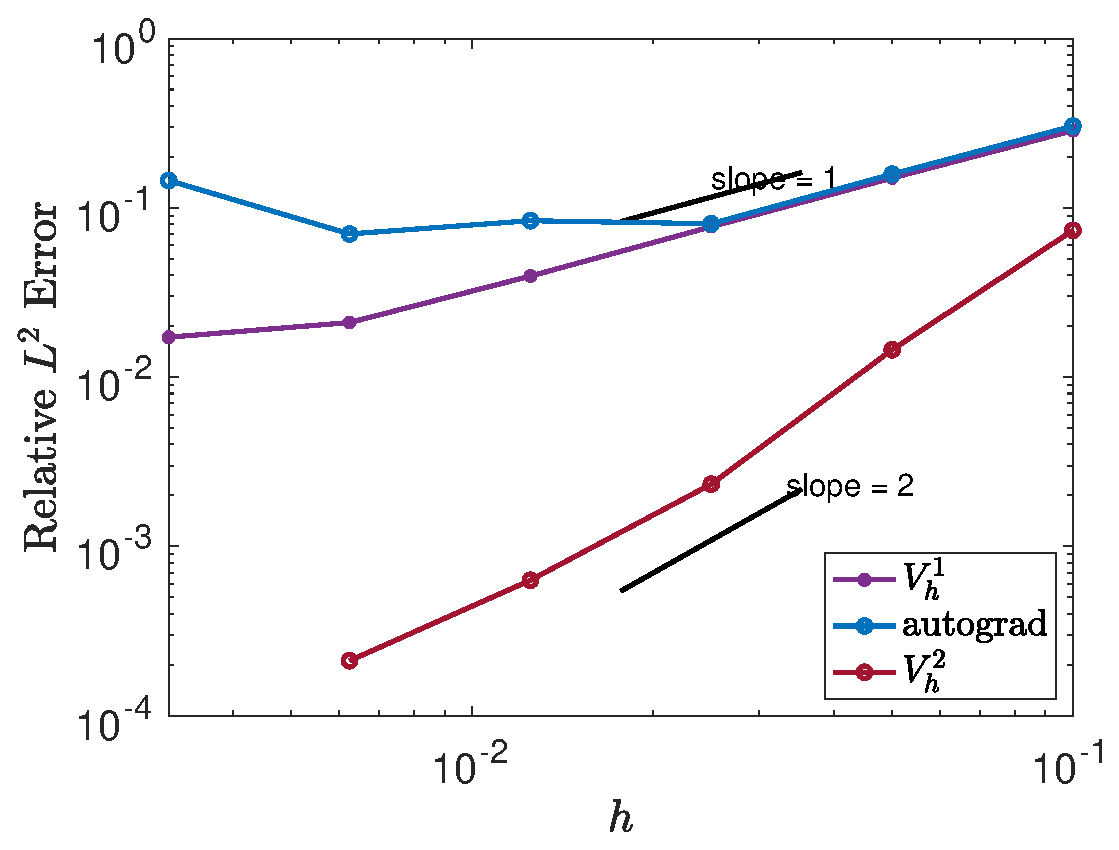
\includegraphics[width=0.7\linewidth]{Figure/Figure_linear_cv}
	\label{fig:1D_conservation_law}
    \end{figure}
\end{frame}

\begin{frame}{Burgers' Equation}

\begin{equation*}
 	u_t + (\frac{u^2}{2})_x = 0
 \end{equation*} 
with initial condition 
 \begin{equation*}
 	u(0,x) = \left\{
 	\begin{matrix}
 		1 & x<0\\
 		 0 & x>0
 	\end{matrix}
 	\right.
 \end{equation*}
and reflecting boundary condition

\medskip

Numerical solution
\begin{equation*}
\begin{aligned}
u(t,x) = \left\{\begin{matrix}
&\mathcal{N}_\theta(t,x_{i+\frac{1}{2}}) \varphi_i(x) &  t > 0 \; x\in(x_i,x_{i+1})\\
&u(0,x_{i+\frac{1}{2}}) &  t = 0 \\
\end{matrix}\right.
\end{aligned}
\end{equation*}

\end{frame}

\begin{frame}{Loss function}
Semi-discrete scheme
\begin{multline*}
\mathcal{L}_{\mathrm{semi}}(\theta) =  \sum_{i,j} \bigg( \frac{\partial u_{\theta}(t_j,x_{i+\frac{1}{2}})}{\partial t} - \hat{f}^{\mathrm{God}}(u_{\theta}(t_j,x^-_i),u_{\theta}(t_j,x^+_i)) \\
+\hat{f}^{\mathrm{God}}(u_{\theta}(t_j,x^-_{i+1}),u_{\theta}(t_j,x^+_{i+1}))  \bigg)^2
\end{multline*}
Fully-discrete scheme using the forward Euler method
\begin{multline*}
\mathcal{L}_{\mathrm{FE}}(\theta) = \sum_{i,j} \bigg( \frac{u_{\theta}(t_{j+1},x_{i+\frac{1}{2}})-u_{\theta}(t_j,x_{i+\frac{1}{2}})}{\Delta t} - \hat{f}^{\mathrm{God}}(u_{\theta}(t_j,x^-_i),u_{\theta}(t_j,x^+_i)) \\
+\hat{f}^{\mathrm{God}}(u_{\theta}(t_j,x^-_{i+1}),u_{\theta}(t_j,x^+_{i+1}))  \bigg)^2
\end{multline*}
\end{frame}

\begin{frame}{Approximation error}
\begin{table}[H]
 \centering
 \begin{tabular}{|c|c|c|c|c|}
 \hline
     $h=\Delta t$ & Fully discrete     & Semi-discrete \\
 	\hline
	1/10 & 9.87 e-02  &  3.82 e-01\\
    1/20 & 4.88 e-02  &  3.37 e-01\\
    1/40 & 3.48 e-02  &  3.03 e-01\\
	1/80 & 2.58 e-02  &  3.12 e-01\\
	1/160& 1.84 e-02  &  1.91 e-01\\
	1/320& 1.73 e-02  &  3.86 e-01\\
\hline
 \end{tabular}
 \caption{The averaged $L^2$ relative error and the convergence rate for the Burgers' equation. Batchsize: $10000$; Width 20, Depth:4, Total number of parameters: $1341$.}
 \end{table}

\end{frame}

\begin{frame}{Solution profiles}
 \begin{figure}[H]

	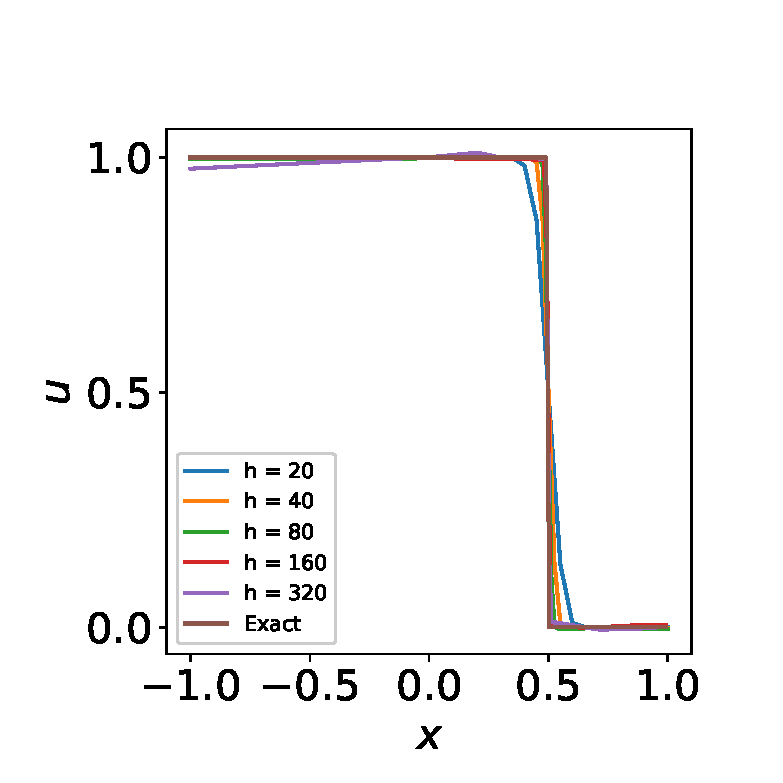
\includegraphics[width=0.4\linewidth]{Figure/Burgus_equation_numerical_100}
\end{figure}
\end{frame}

\begin{frame}{Stochastic linear conservation law}

\begin{equation*}
	\begin{aligned}
		2 d  \pi u_t  - (1+\exp((-\sum_{j=1}^s \omega_j)^2)) \sum_{i} u_{x_i}  = 0 
	\end{aligned}
\end{equation*}
with periodic boundary condition and initial condition $u(0,\boldsymbol{x},\boldsymbol{\omega}) = g(\boldsymbol{x}) =  \sin\left(2\pi \sum_{i=1}^d x_i \right) $ 

\medskip
Exact solution $u(t,\boldsymbol{x},\boldsymbol{\omega}) = \sin\left((1+\exp ( (-\sum_{j=1}^s \omega_j)^2) ) t + 2\pi \sum_{i=1}^d x_i\right)$

\medskip
Numerical solution
\begin{equation*}
\begin{aligned}
&u(t,\boldsymbol{x},\boldsymbol{\omega}) = \sum_{\boldsymbol{i}} [t\mathcal{N}_\theta(t,\boldsymbol{x}_{\boldsymbol{i}+\frac{1}{2}},\boldsymbol{\omega}) + g(\boldsymbol{x}_{\boldsymbol{i}+\frac{1}{2}} )]\varphi_{\boldsymbol{i}}(\boldsymbol{x})
\end{aligned}
\end{equation*}

\end{frame}

\begin{frame}{Loss function}

\begin{multline*}
\mathcal{L}_{\mathrm{FE}}(\theta) = \sum_{i,j}\bigg(2\pi \frac{ u_{\theta}(t_{j+1},\boldsymbol{x}_{\boldsymbol{i}+\frac12},\boldsymbol{\omega}) - u_{\theta}(t_j,\boldsymbol{x}_{\boldsymbol{i}+\frac12},\boldsymbol{\omega})}{\Delta t} \\
- (1+\exp(-\sum_{j=1}^s \omega_j)^2) \frac{u_{\theta}(t_j,\boldsymbol{x}_{\boldsymbol{i}+1},\bom) -u_{\theta}(t_j,\boldsymbol{x}_{\boldsymbol{i}},\boldsymbol{\omega})}{h} \bigg)^2
\end{multline*}

\begin{table}[ht]
 \centering
 \begin{tabular}{|c|c|c|c|c|c|c|}
 \hline
     $s$ & $h = \Delta t$ &  Expectation & Order & Variance  & Order\\
 	\hline
	 100 & 1/40 & 1.53 e-01 &  & 2.07 e-01 & \\
	 100 & 1/80 & 7.83 e-02 & 0.97 &  1.12 e-01 & 0.88\\
	 100 & 1/160 & 3.93 e-02 & 0.99 & 5.82 e-02 & 0.95\\
	 100 & 1/320 & 2.01 e-02 & 0.96 &  2.93 e-02 & 0.98\\
\hline
 \end{tabular}
\label{tbl:cv error stochastic}	
\end{table}
\end{frame}

\begin{frame}{Solution profiles}
\begin{figure}[htbp]
\centering
	\subfigure[$s=5$]{
		\includegraphics[width=0.45\linewidth]{Figure/CL_equation_storchstic_dim_s_100_E.eps}
	}
	\subfigure[$s=5$]{
		\includegraphics[width=0.45\linewidth]{Figure/CL_equation_storchstic_dim_s_100_V.eps}
	}
\end{figure}
\end{frame}

\begin{frame}{Stochastic Burgers' equation}

\begin{equation*}
 	u_t + (\frac{u^2}{2})_x = 0
 \end{equation*} 
with initial condition 
 \begin{equation*}
 	u(0,x,\boldsymbol{\omega}) = \left\{
 	\begin{matrix}
 		1+\epsilon \sum_{i=1}^s \omega_i & x<0 \\
 		 0 & x>0 
 	\end{matrix}
 	\right.
 \end{equation*}
Exact solution
\begin{equation*}
	 	u(t,x,\boldsymbol{\omega}) = \left\{
 	\begin{matrix}
 		z  & x< \frac{z}{2}\\
 		 0 & x>\frac{z}{2}
 	\end{matrix}
 	\right.
\end{equation*}
where $z = 1+\eps \sum_{i=1}^s \om_i$
\end{frame}

\begin{frame}{DNN solution}
 \begin{equation*}
 \begin{aligned}
 	u(t,x,\boldsymbol{\omega}) = \left\{\begin{matrix}
 		&\mathcal{N}_\theta(t,x_{i+\frac{1}{2}},\boldsymbol{\omega}) \varphi_i(x) &  t > 0 \; x\in(x_i,x_{i+1})\\
 		&u(0,x_{i+\frac{1}{2}},\boldsymbol{\omega}) &  t = 0 \\
 	\end{matrix}\right.
\end{aligned}
 \end{equation*}
\end{frame}

\begin{frame}
\footnotesize
\begin{table}[htbp]
	\centering
	\begin{tabular}{|c|c|c|c|c|c|c|}
		\hline
		\multirow{2}*{$\eps$} & \multirow{2}*{$s$}  &\multirow{2}*{$h$}   & \multicolumn{2}{c|}{$L^2$ error}            & \multicolumn{2}{c|}{$L^1$ error}  \\
		\cline{4-7}
		~ &~ & ~ & Expectation & Variance & Expectation & Variance \\
		\hline
%		0.25 & 2 & 1/40  &  2.44 e-3 & 1.27 e-1 & 1.63 e-03 & 8.66 e-02\\
%		0.25 & 2 & 1/80  &  3.57 e-3 & 8.82 e-2 & 2.06 e-03 & 5.77 e-02\\
%		0.25 & 2 & 1/160 &  9.70 e-3 & 1.14 e-1 & 4.42 e-03 & 7.40 e-02\\
%		0.25 & 2 & 1/320 &  2.28 e-2 & 2.21 e-1 & 1.10 e-02 & 1.46 e-01\\
%		0.1  & 5 & 1/40  &  4.16 e-3 & 2.30 e-1 & 2.03 e-03 & 1.60 e-01\\
%		0.1  & 5 & 1/80  &  2.44 e-3 & 1.24 e-1 & 1.34 e-03 & 9.78 e-02\\
%		0.1  & 5 & 1/160 &  4.34 e-3 & 9.16 e-2 & 2.17 e-03 & 8.04 e-02\\
%		0.1  & 5 & 1/320 &  1.61 e-2 & 2.21 e-1 & 8.10 e-03 & 1.75 e-01\\
		0.05 & 10 & 1/40 & 6.79 e-3 & 3.37 e-1  & 2.99 e-03 & 2.40 e-01\\
		0.05 & 10 & 1/80 & 2.25 e-3 & 1.86 e-1  & 1.13 e-03 & 1.45 e-01\\
		0.05 & 10 & 1/160 & 4.68 e-3 & 1.27 e-1 & 2.28 e-03 & 1.17 e-01 \\
		0.05 & 10 & 1/320 & 2.01 e-2 & 3.36 e-1 & 8.94 e-03 & 2.74 e-01\\
		0.01 & 50 & 1/40 & 1.80 e-2 & 6.42 e-1  & 5.36 e-03 & 5.01 e-01\\
		0.01 & 50 & 1/80 & 5.74 e-3 & 4.04 e-1 & 1.67 e-03 & 3.32 e-01\\
		0.01 & 50 & 1/160 & 3.09 e-3 & 2.69 e-1 & 1.18 e-03 & 2.68 e-01\\
		0.01 & 50 & 1/320 & 4.40 e-2 & 9.12 e-1 & 1.70 e-02 & 8.06 e-01\\
		0.005 & 100 & 1/40 & 2.58 e-2 & 7.53 e-1 & 6.54 e-03 & 5.01 e-01\\
		0.005 & 100 & 1/80 & 8.64 e-3 & 5.25 e-1 & 2.09 e-03 & 3.32 e-01\\
		0.005 & 100 & 1/160 & 1.95 e-3 & 3.76 e-1& 7.22 e-04 & 2.68 e-01\\
		0.005 & 100 & 1/320 & 3.07 e-2 & 9.47 e-1& 5.65 e-03 & 8.06 e-01\\
		0.0025 & 200 & 1/40 & 2.58 e-2 & 7.53 e-1 & 7.56 e-03 & 7.52 e-01\\
		0.0025 & 200 & 1/80 & 8.64 e-3 & 5.25 e-1 & 2.51 e-03 & 5.68 e-01\\
		0.0025 & 200 & 1/160 & 1.95 e-3 & 3.76 e-1 & 8.30 e-04 & 5.51 e-01\\
		0.0025 & 200 & 1/320 & 3.07 e-2 & 9.47 e-1 & 3.52 e-03 & 9.09 e-01\\
		\hline
	\end{tabular}
	\caption{Expectation and variance errors of the proposed method for the stochastic Burgers' equation when the MC method is used with the batchsize $50000$.}
	\label{tbl: s Bur equation 50000 eroor}
\end{table}
\end{frame}
\begin{figure}
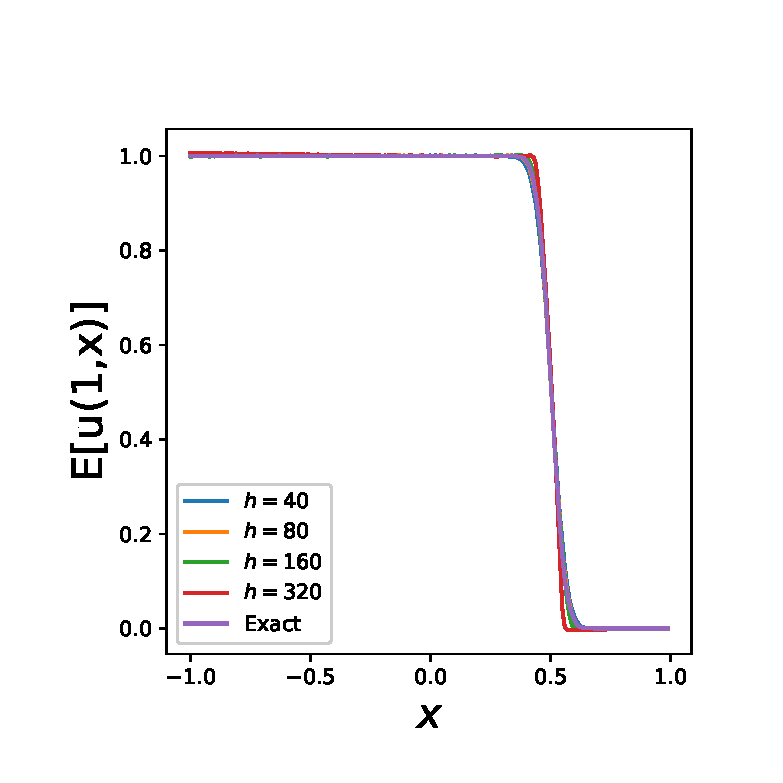
\includegraphics[width = 0.4\linewidth]{Figure/Burgus_equation_storchstic_dim_s_10_eps_005_E}
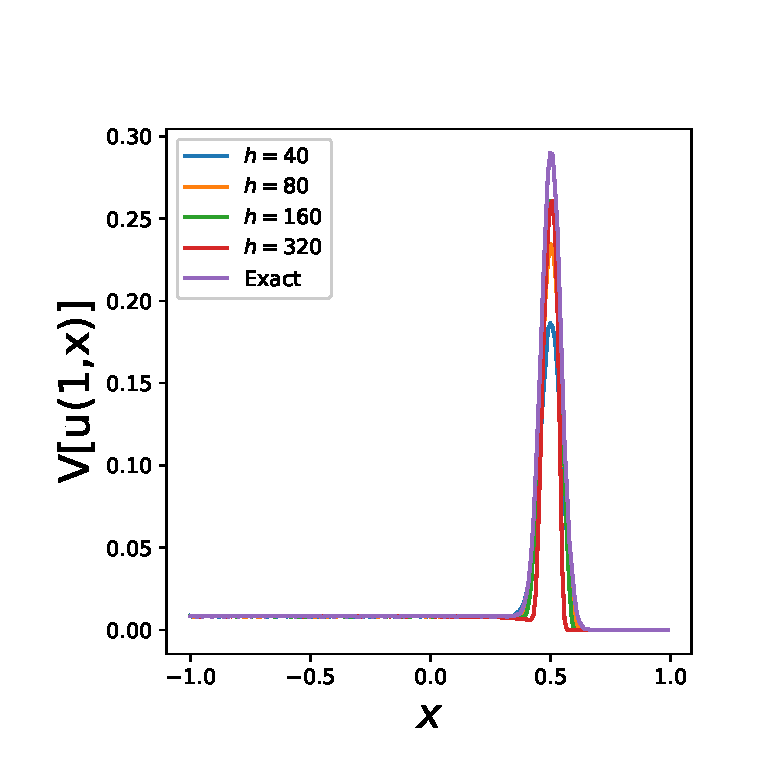
\includegraphics[width = 0.4\linewidth]{Figure/Burgus_equation_storchstic_dim_s_10_eps_005_V}
\end{figure}
\begin{frame}
\frametitle{Conclusion}

{\huge\medskip
	\begin{center}
		\textcolor{red}{Discretize-then-learn}
	\end{center}
}
\begin{itemize}
	\item A stable and convergent scheme in the classical sense
	\item A neural network representation of the numerical solution
	\item A loss function in the least-squares sense
	\item Monte-Carlo sampling
\end{itemize}

{\huge\medskip
	\begin{center}
		\textcolor{blue}{Thank you for your attention!}
	\end{center}
}
\end{frame}
\end{document}

